\documentclass[12pt,a4paper]{article} 
\usepackage[utf8]{inputenc} 
\usepackage[russian]{babel} 
\usepackage{amsmath} 
\usepackage{amsfonts} 
\usepackage{euscript} 
\usepackage{amssymb} 
\usepackage{makeidx} 
\usepackage[left=1cm, right=1cm, top=1cm, bottom=2cm]{geometry} 
\author{Богатый Антон} 
\title{Алгоритм Холецкого.} 
\usepackage{graphicx}
\begin{document}
\begin{center}
\textbf{Поиск обратной матрицы с помощью блочного метода Холецкого.}
\end{center}
\textit{Теоретическая основа метода:}
\\
\indent В случае обычного метода Холецкого, мы ищем представление симметричной матрицы
$A$ в виде $A = R^t * D * R$, где $R$ - верхнетреугольная положительно опеределенная матрица, 
а $D$ - диагональная матрица с ${\pm}1$ на диагонали. Исходя из такого разложения не сложно получить формулы
для вычисления элементов матриц $D$ и $R$:
$$d_{i i} = sgn({a_{i i} - \sum_{k=1}^{i-1} {r_{k i}^2 * d_{k k}}})$$ 
$$r_{i i} = \sqrt{\vert a_{i i} - \sum_{k=1}^{i-1} r_{k i}^2 * d_{k k} \vert}$$
$$r_{i j} = \dfrac{a_{i j} - \sum_{k=1}^{i-1} r_{k i} * d_{k k} * r_{k j}}{r_{i i} * d_{i i}}$$

\indent Но если мы хотим эффективно использовать ресурсы кэш памяти процессора, то нам необходимо представить матрицы $A, R, D$ в блочном виде и оперировать с блоками, тогда в случае $A = (A_{i j})$, $R = (R_{i j})$ формулы примут следующий вид:
$$ A_{i j} = \sum_{k = 1}^{l} {(R^{t})_{i k} * D_{k k} * R_{k j}} = 
\sum_{k = 1}^{i} {R^{t}_{k i} * D_{k k} * R_{k j}} $$  
Отсюда получаем формулы для пересчета $R_{i i}$ и $D_{i i}$:
$$R^t_{i i} \cdot D_{i i} \cdot R_{i i} = A_{i i} - \sum_{k=1}^{i-1} R_{k i}^t * D_{k k} * R_{k i} $$
\indent Заметим, что правая часть равенства - симметричная матрица, т.е. $R_{i i}$ - это верхнетреугольная матрица из разложения Холецкого правой части, которое мы уже умеем вычислять не в блочном случае, а $D_{i i}$ - диагональная матрица из разложения. После получения $ R_{i i} $ можно приступить к вычислению $R_{i j}$:
$$R_{i j} = D_{i i}^{-1} * R_{i i}^{-1}*(A_{i j} - \sum_{k=1}^{i-1} R_{k i}^t * D_{k k} * R_{k j}) $$
\indent Здесь мы рассмотрели строчный вариант метода Холецкого, где $R_{i j}$ вычисляются по строкам. Проведя расчеты по этим формулам, мы получим верхнетреугольную матрицу R, к такой матрице обратная матрица легко ищется последовательным исключением строк. Тогда искомая матрица $ A^{-1} $ будет иметь вид: $A^{-1} = R^{-1} * D^{-1} * ({R^{-1}})^t$.
\\
\begin{center}
\textbf{Параллельная версия блочного метода Холецкого на MPI.}
\end{center}
Блочный алгоритм мы рассмотрели, далее мы считаем каждый блок единичным неделимым элементом, т.e. мы получаем матрицу размером $n \cdot n$, где $n = \lceil \frac{N}{M} \rceil$, $N$ - размер матрицы, $M$ - размер блока. Дальше будем рассматривать только симметричные положительно определенные матрицы $A$, тогда $A$ можно представить в виде $A = R \cdot R^{T}$, где $R$ - нижнетреугольная положительно определенная матрица.
\\
\indent \textit{Разбиение матрицы по процессорам:}
\\
Процессор номер $i$ будет хранить строки с номерами 
$i, i + P, i + 2 \cdot P, ...$, где $P$ - общее количество процессоров.
Для $n=5$ и $P=3$ разбиение примет вид:
\\
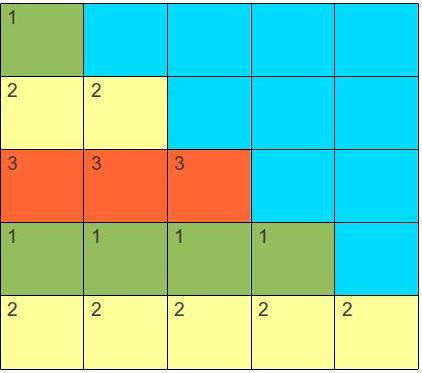
\includegraphics[width=64mm]{img0.jpg}
\\
Из разложения $A = R \cdot R^T$ ясно, что
$$r_{j i} \cdot r_{i i}^T = a_{j i} - \sum_{k=1}^{i-1}{r_{j k} * r_{i k}^T} ~, i < j ~ ~ ~ ~ ~ ~ ~ (*) $$
Будем вычислять матрицу $R$ по столбцам, т.е. на $i$-м шаге будем вычислять $i$-ый столбец. Причём $j$-ый процессор будет вычислять $r_{j i}$, т.е. тот элемент, который находится у него в памяти. Для того, чтобы воспользоваться формулой $(*)$ нужна ещё $i$-ая строка, которая будет разослана всем процессорам на $i$-м шаге. Совершенно аналогично поступим и при обращении матрицы $R$, а именно правая часть будет разбита по процессорам так же.
\\
\indent \textit{Вычисление произведения матриц:}
\\
Теперь вычислим $A^{-1} = R^{-T} \cdot R^{-1}$, поскольку матрица $A$ - симметричная, то каждый элемент матрицы $A$ - это произведение 2-х строк матрицы $R^{-T}$. Будем делать так - по одной строке рассылаем на все процессоры, где она умножается на все строки, которые хранятся в этом процессоре.
\\
\indent \textit{Количество и объём пересылок:}
\\
1) Разложение Холецкого:
\\
Количество: $n = \frac{N}{M}$
\\
Объём: $\sum_{i = 1}^{n} {i \cdot M^2} \simeq \frac{N^2}{2} $
\\
2) Обращение матрицы $R$:
\\
Количество: $n = \frac{N}{M}$
\\
Объём: $\sum_{i = 1}^{n} {i \cdot M^2} \simeq \frac{N^2}{2} $
\\
3) Перемножение матриц $R^{-1} \cdot R^{-T}$:
\\
Количество: $2 \cdot n = 2 \cdot \frac{N}{M}$
\\
Объём: $2 \cdot \sum_{i = 1}^{n} {i \cdot M^2} \simeq N^2 $
\end{document}